\newpage
\section{Results \& Analysis}

\subsection{Ideal Gas: Results}
\label{Ideal Gas Results}

When inserting the metal can into the thermal baths and starting a measurement, the pressure either abruptly spiked or shrank. The pressure graph then met its extreme value and due to leakage, it quickly rebound to pressure at room temperature, as seen in Figure \ref{fig:P-time graph comp (cold vs hot)}. The extreme value is chosen as the desired value for the given temperature. 

\begin{figure}[H]
    \centering
    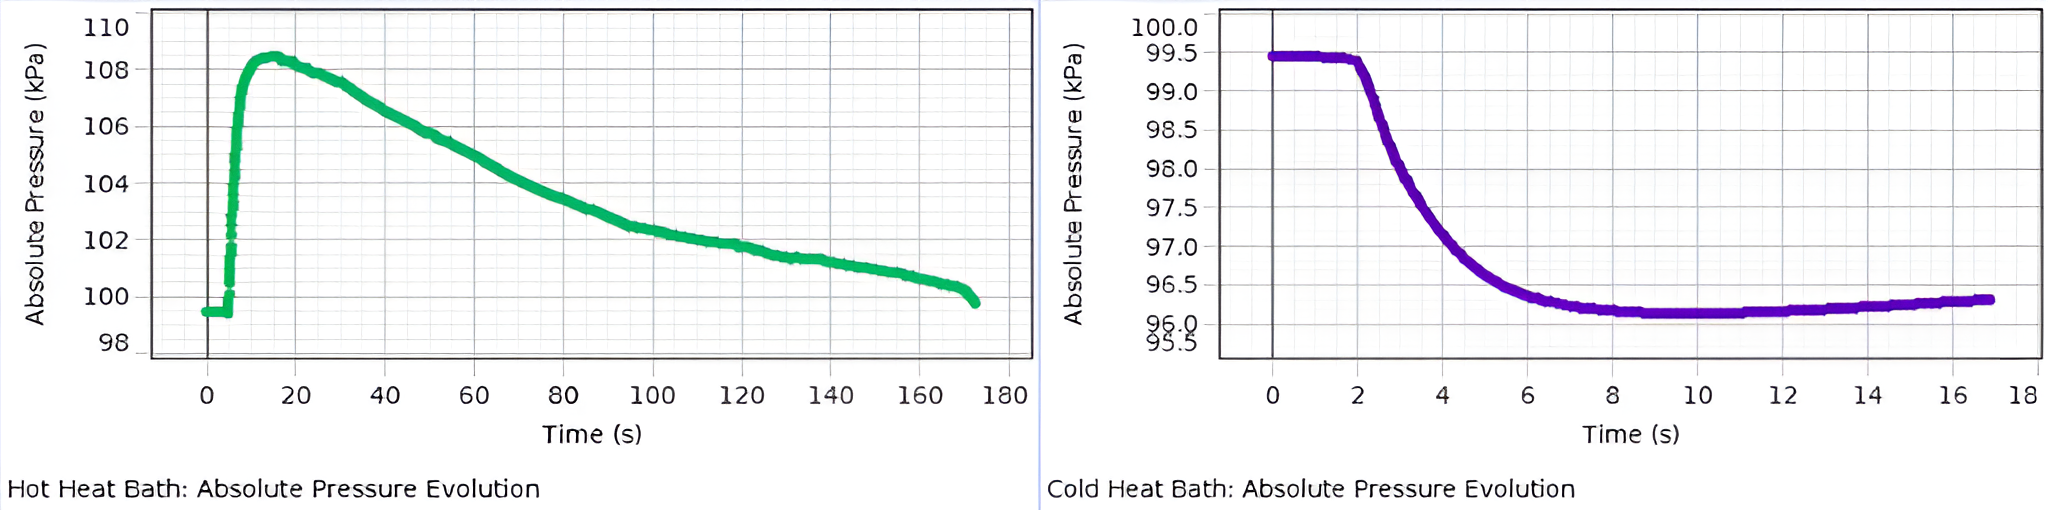
\includegraphics[width=1\linewidth]{Graphics/P_Evolution.png}
    \caption{Evolution of Pressure inside the system over time. Left: Pressure increases after inserting the can into a hot reservoir, the pressure used corresponds to the maximum. Right: Pressure decreases after inserting the can into a cold reservoir, the pressure used corresponds to the minimum.}
    \label{fig:P-time graph comp (cold vs hot)}
\end{figure}

Some fluctuations occurred at the begin of the data logging process, which affected the temperature inside the system. The temperature values will therefore possess additional uncertainties due to lack of knowledge about the precise value. Compiling all runs:

\begin{table}[H] 
    \setlength{\tabcolsep}{8pt} % Adjust column separation for clarity
    \renewcommand{\arraystretch}{1.3} % Adjust row height for better spacing
    \centering
    \small % Smaller font size
    \begin{tabular}{|c >{\centering\arraybackslash}p{4cm}|} % Set specific width for all columns
    \hline
     \textbf{Pressure [kPa]} &  \textbf{Temperature [\degree C]} \\ \hline \hline
    95.135 & $9.978 \pm 0.516$ \\ \hline
    100.808 & $29.125 \pm 0.510$ \\ \hline
    104.218 &  $42.250 \pm 0.515$ \\ \hline
    108.500 & $63.989 \pm 0.550$ \\ \hline
    \end{tabular}
    \caption{Checking Gay-Lussac's Law: Temperature against Pressure measurements from the various heat baths.}
    \label{tab:Ideal_Gas_Law}
\end{table}

For air to be an ideal gas, it must obey Gay-Lussac's Law, which declares a linear correlation between temperature and pressure when other variables are held constant. The data from Table \ref{tab:Ideal_Gas_Law} are therefore plotted, fitting a linear function of type $\mathit{Ax + B}$. The result is shown in Figure \ref{fig:P-time}.


\begin{figure}[H]
    \centering
    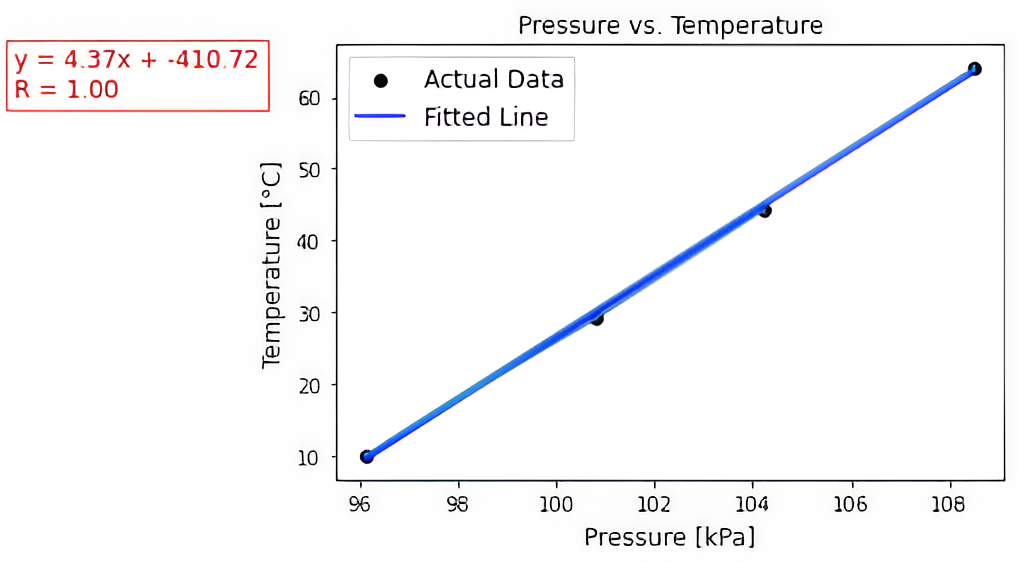
\includegraphics[width=0.5\textwidth]{Graphics/Ideal_Gas_plot.png}
    \caption{Checking Gay-Lussac's Law: Graph plotting Pressure vs Temperature. A linear function is fitted to the graph, with a correlation coefficient of $\mathit{R=1}$.}
    \label{fig:P-time}
\end{figure}

The linear correlation is verified, with a correlation coefficient of $\mathit{R = 1.00}$. One can therefore proceed with the ensuing experiment.

\subsection{Thermodynamic Cycle: Results}
\label{Therm Cycle Results}

The cycle of the first data run was chosen for analysis. A PV-diagram of the collected data is depicted in Figure \ref{fig:Cycle_Exp}. Some points had to be deleted, as Capstone could not properly connect certain points. This had been due to the frequencies of the Rotary Motion Sensor and Pressure Sensor being different, where 5 pressure values were found for every 2 position values. 

Nonetheless, the total work could properly estimated as $\mathit{W = 0.0618 J}$.

\begin{figure}[H]
    \centering
    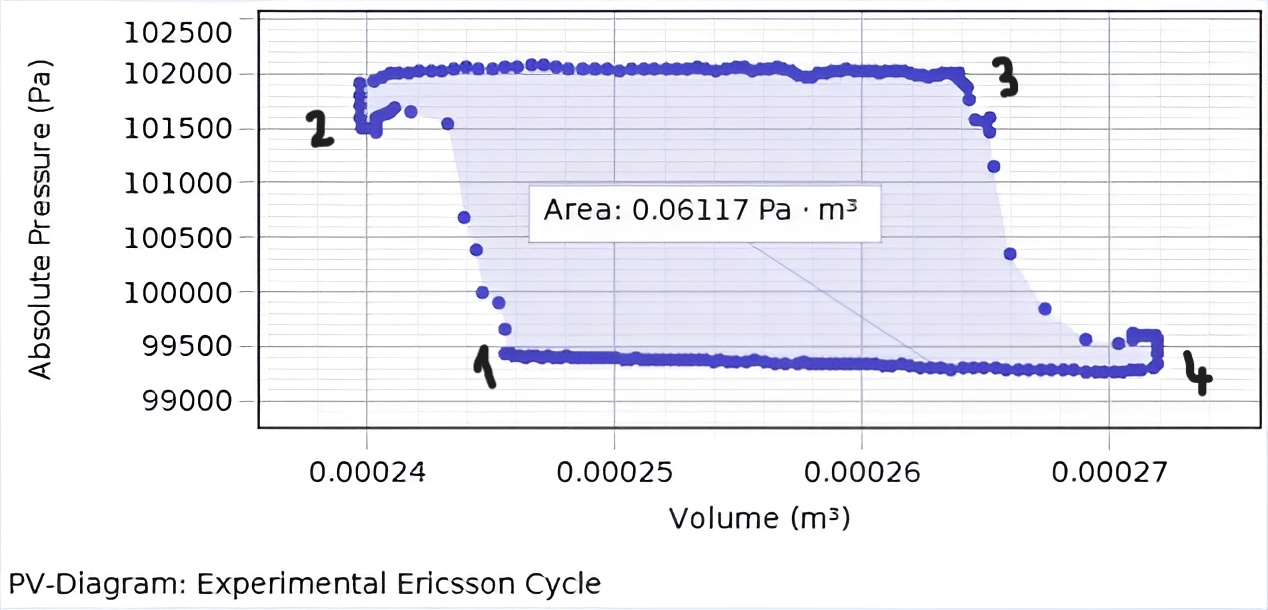
\includegraphics[width=0.6\linewidth]{Graphics/PV-Diagram_Ericsson.png}
    \caption{PV-Diagram of the simulated quasi-Ericsson Cycle. The process is initiated at equilibrium point 1, and cycles over 4 thermodynamic processes back to its original position. The area inside the graph represents the work per cycle.}
    \label{fig:Cycle_Exp}
\end{figure}

Temperatures of the baths were given by $\mathit{T_1 = T_2 = T_c = (284.285 \pm 0.500) K}$ for the cold reservoir and $\mathit{T_4 = T_3 = T_h = (324.758 \pm 0.500) K} $ for the hot one. The temperatures stayed constant over the isothermal paths. Furthermore, equilibrium point 1 corresponds to the initial position, with a volume of $\mathit{V_1 = \pi r_p^2 y_0 + V_{can} + V_{pipes} \approx (2.458 \pm 0.025) \cdot 10^{-4} m^3}$. 

% pressure errors by looking at the deviations along the cosntant line

The cycle consisted of two isobaric processes. To assess the corresponding pressures, an average of the values between equilibrium points 2 and 3 as well as 4 and 1 was determined, with the approximate deviations from the constant line representing the uncertainties. For further calculation $\mathit{P_2 = P_3 = (102011 \pm 25) Pa}$ and $\mathit{P_1 = P_4 = (99290 \pm 75) Pa}$ are utilized.

During process IV, between points 4 and 1, the ratio $\mathit{\frac{V}{T}}$ stayed constant. As a result, $\mathit{V_4}$ can also be expressed as:

\begin{equation}
\label{eq:V_4}
    \mathit{V_4 = V_1 \frac{T_h}{T_c}}
\end{equation}

Furthermore, the isothermal process III between points 3 and 4 implied that for that duration, $\mathit{PV = const}$. $\mathit{V_3}$ can thus be written as:

\begin{equation}
\label{eq:V_3}
    \mathit{V_3 = V_4 \frac{P_4}{P_3}}
\end{equation}

These relation can be implemented when calculating the heat absorbed during the cycle. For process II, Equation \ref{eq:Q_II} will be used for the calculations:
% error on pressure negligible

\begin{equation}
\label{eq:V_T const}
    \mathit{Q_{II} = \frac{7}{2} \frac{P_4 V_4}{T_h}(T_h - T_c) \approx (11.8545 \pm 0.3186) J}
\end{equation}

The errors included above are governed by the error propagation of all variables included in the formula. Noting that the error in pressure can be neglected, the relative error is given by Equation \ref{eq:Q_II_Error}:

\begin{equation}
    \label{eq:Q_II_Error}
    \mathit{\frac{\Delta Q_{II}}{Q_{II}} = \sqrt{(\frac{\varepsilon_{V_4}}{V_4})^2 + (\frac{\varepsilon_{T_h}}{T_h})^2 + (\frac{\varepsilon_{T_h} + \varepsilon_{T_c}}{T_h -T_c})^2} \approx 0.0269}
\end{equation} 

A similar procedure can be conducted for the isobaric process III:

\begin{equation}
\label{eq:T const}
    \mathit{Q_{III} = P_4 V_4 \ln{\frac{V_4}{V_3}} \approx (0.7514 \pm 0.5033) J}
\end{equation}

Here, the error is also gained from analyzing the error propagation. Noting that the error for a function of type $\mathit{\ln{x}}$ is $\mathit{\Delta \ln{x} \approx \frac{\Delta x}{x}}$, and $\mathit{\ln{\frac{V_4}{V_3}} = \ln{V_4} - \ln{V_3}}$: 

\begin{equation}
    \label{eq:Q_III_Error}
    \mathit{\frac{\Delta Q_{III}}{Q_{III}} = \sqrt{(\frac{\varepsilon_{V_4}}{V_4})^2 + (\frac{\frac{\varepsilon_{V_4}}{V_4} + \frac{\varepsilon_{V_3}}{V_3}}{lnV_4-lnV_3})^2} \approx 0.6698}
\end{equation}

The high uncertainty can be traced back to the small difference between the volumes, causing the logarithmic function to be sensitive to small changes.

Equation \ref{eq:Q_tot} portrays the total heat absorbed in the process.

\begin{equation}
\label{eq:Q_tot}
    \mathit{Q_{h} = Q_{II} + Q_{III} = (12.6059 \pm 0.8219) J}
\end{equation}

Finally, one can insert the values for work $\mathit{W}$ and heat $\mathit{Q_h}$ to find the heat engine's actual efficiency:

\begin{equation}
\label{eq:Exp_Efficiency}
    \mathit{\nu = \frac{W}{Q_h} \approx 0.00485 \pm 0.00032}
\end{equation}

If the cycle were that of an ideal Carnot Cycle, the efficiency would instead be the one calculated below:

\begin{equation}
\label{eq:Exp_Carnot_Efficiency}
    \mathit{\eta =  1-\frac{T_c}{T_h} \approx 0.12186 \pm 0.00028}
\end{equation}

One can see that the maximum efficiency of the engine is clearly not reached by the conducted cycle. In fact, the engine only works at approx. $\mathit{3.98 \%}$ of its ideal thermodynamical efficiency.